\section{Experiments}\label{sec:exps}

\subsection{Experimental Setup}
The SPO algorithm is broadly applicable in LLM reasoning tasks~\cite{R1} and Agentic training. We evaluate Tool-Integrated Reasoning (TIR)~\cite{feng2025retool,aspo} scenarios, where the LLMs can utilize external Python interpreter to help solve hard problems. We conduct experiments using a moderately sized LLM, Qwen3-8B~\cite{qwen3}. 
For training data, we use the English subset from the DAPO dataset~\cite{DAPO}. Only outcome reward is applied for RLVR, without the format rewards. We evaluate performance on the challenging math competition benchmarks, i.e., AIME 24, AIME 25, BeyondAIME~\cite{seed1.5}, BRUMO 25~\cite{matharena}, and HMMT 25~\cite{matharena}. 
See Appendix~\ref{appendix:training_details} for training and evaluation details.



We distinguish our goal from that of ``hill-climbing'' on benchmark leaderboards. The latter often necessitates resource-intensive and highly specialized techniques, including SFT from frontier models~\cite{liu2025acereason11}, mid-training~\cite{wang2025octothinker}, multi-stage RL pipelines~\cite{deepscaler2025,he2025skywork,chen2025acereason}, curated hard datasets with intricate processing~\cite{Polaris2025, shang2025rstar2}, test-time scaling techniques~\cite{fu2025deep} and extremely large generation group sizes~\cite{zeng2025glm}. Our work, instead, concentrates on the fundamental efficiency and scalability of the RL algorithm itself. 



\subsection{Empirical Comparison with GRPO}

\begin{table}[h!]
\centering
\caption{Comparison of GRPO and SPO on five benchmarks using maj@32 and avg@32. Averages are shown in the last column. Bold indicates the better-performing method for each metric.}
\label{tab:main_results}
\begin{adjustbox}{max width=\textwidth}
\begin{tabular}{lcccccccccccc}
\toprule
\multirow{2}{*}{Method} 
& \multicolumn{2}{c}{AIME 24} 
& \multicolumn{2}{c}{AIME 25} 
& \multicolumn{2}{c}{BeyondAIME} 
& \multicolumn{2}{c}{BRUMO 25} 
& \multicolumn{2}{c}{HMMT 25} 
& \multicolumn{2}{c}{Average} \\
\cmidrule(lr){2-3}
\cmidrule(lr){4-5}
\cmidrule(lr){6-7}
\cmidrule(lr){8-9}
\cmidrule(lr){10-11}
\cmidrule(lr){12-13}
 & maj@32 & avg@32 
 & maj@32 & avg@32 
 & maj@32 & avg@32 
 & maj@32 & avg@32 
 & maj@32 & avg@32 
 & maj@32 & avg@32 \\
\midrule
Qwen3-8B & 77.8 & 64.4 & 70.5 & 58.4 & 45.2 & 38.0 & 55.1 & 49.4 & 36.8 & 30.3 & 57.1 & 48.1 \\
GRPO & 83.3 & \textbf{77.6} & 72.1 & 64.2 & 45.6 & 39.0 & 56.7 & 56.9 & 44.2 & \textbf{40.9} & 60.4 & 55.7 \\
SPO  & \textbf{84.0} & 74.9 & \textbf{76.5} & \textbf{65.0} & \textbf{46.9} & \textbf{40.3} & \textbf{64.0} & \textbf{59.0} & \textbf{47.5} & 40.6 & \textbf{63.8} & \textbf{56.0} \\
\bottomrule
\end{tabular}
\end{adjustbox}
\end{table}




\begin{figure}[h!]
\centering
\resizebox{0.8\linewidth}{!}{%
\begin{minipage}{\linewidth}
\centering

\begin{subfigure}{0.32\textwidth}
  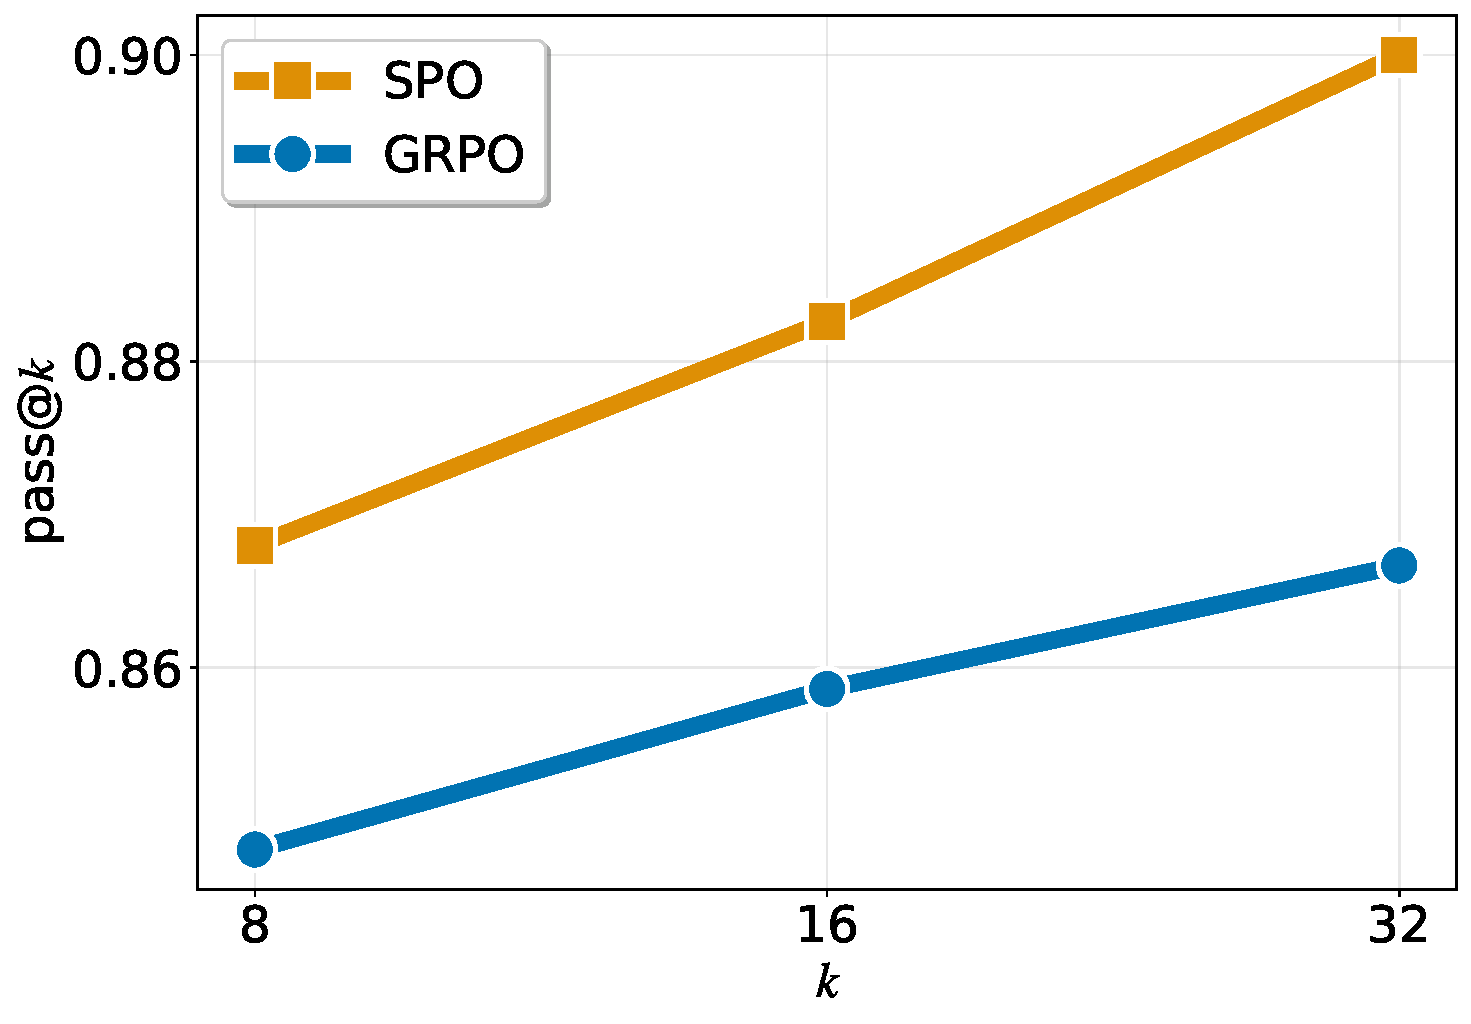
\includegraphics[width=\linewidth]{figures/GRPO_vs_SPO_AIME24_pass_at_k.pdf}
  \caption{AIME 24}
  \label{fig:pass_k_aime24}
\end{subfigure}
\hfill
\begin{subfigure}{0.32\textwidth}
  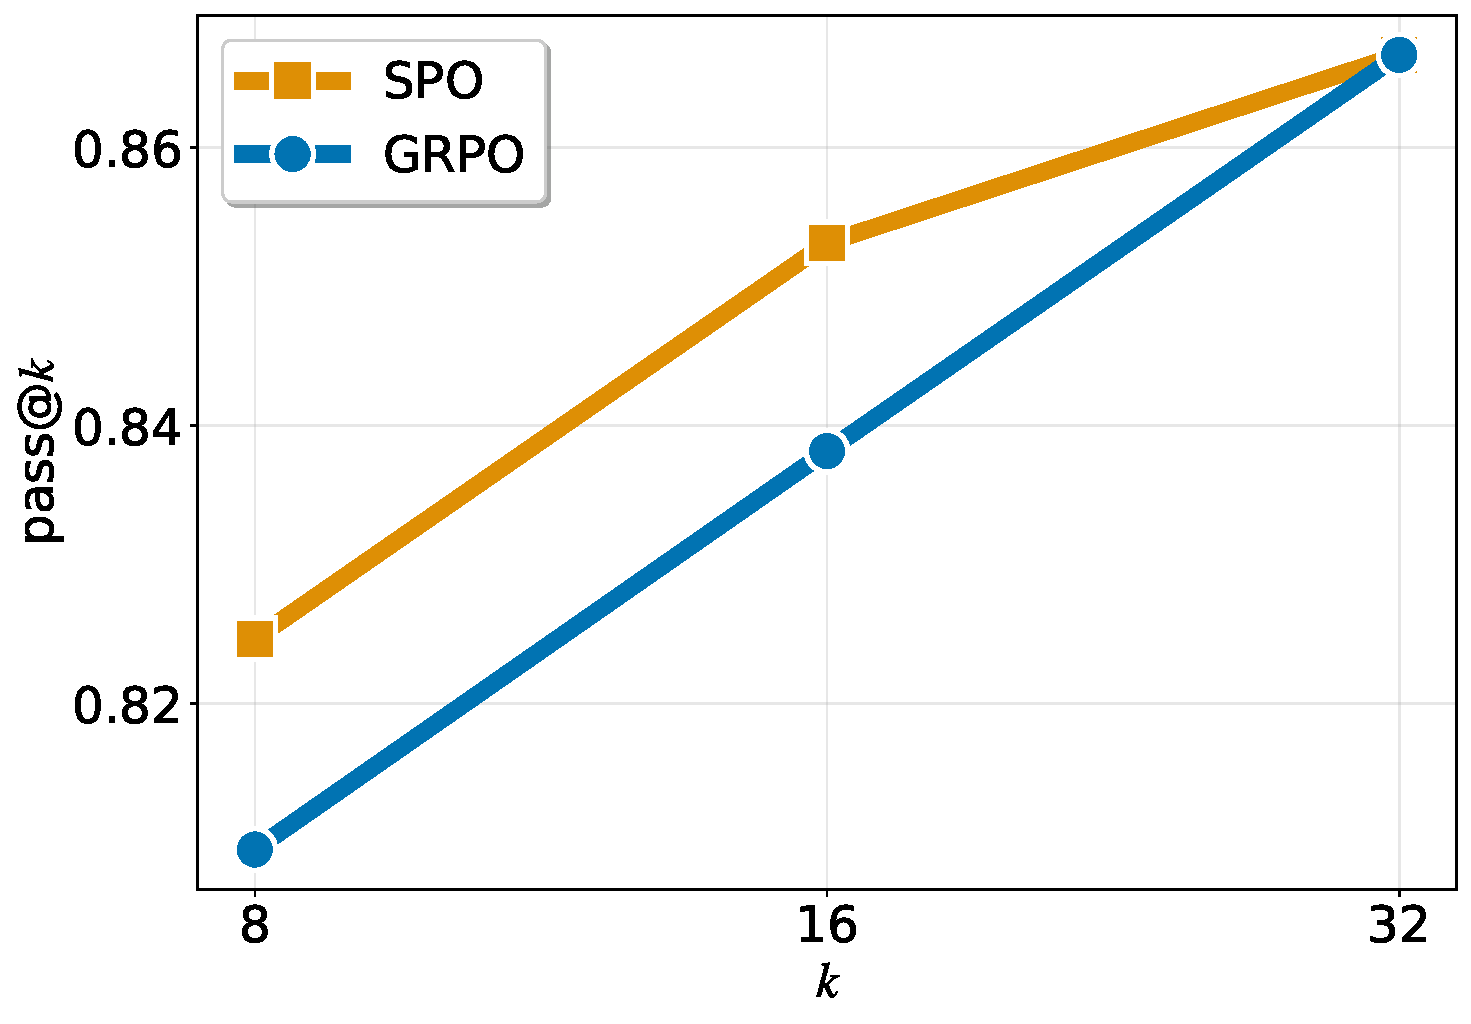
\includegraphics[width=\linewidth]{figures/GRPO_vs_SPO_AIME25_pass_at_k.pdf}
  \caption{AIME 25}
  \label{fig:pass_k_aime25}
\end{subfigure}
\hfill
\begin{subfigure}{0.32\textwidth}
  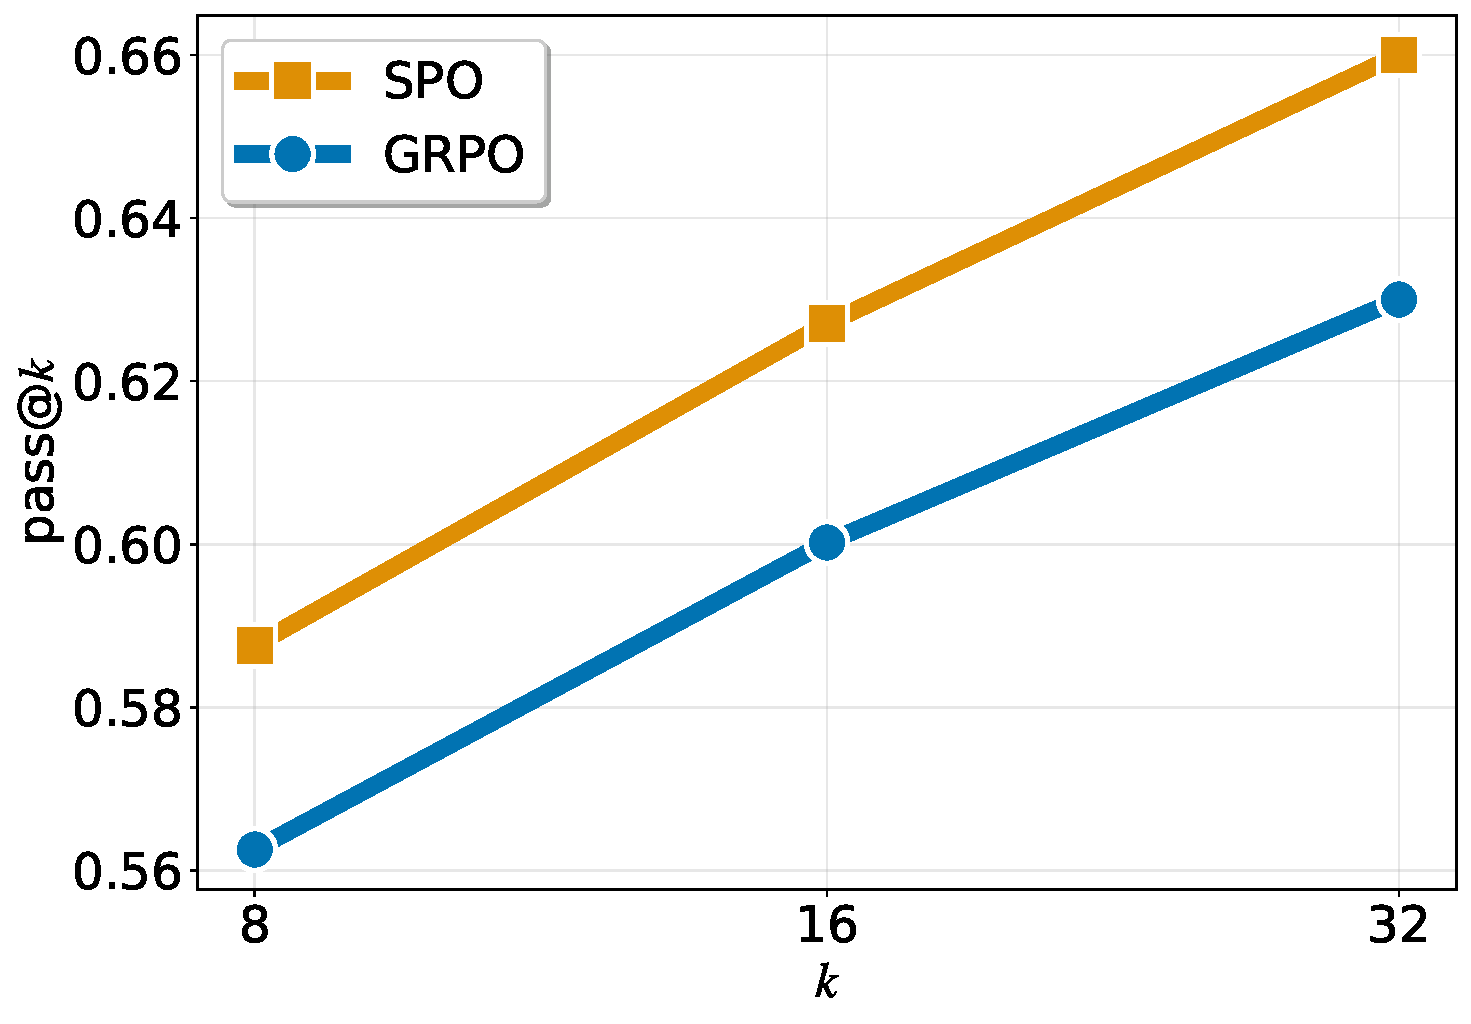
\includegraphics[width=\linewidth]{figures/GRPO_vs_SPO_BeyondAIME_pass_at_k.pdf}
  \caption{BeyondAIME}
  \label{fig:pass_k_beyondaime}
\end{subfigure}
\medskip

\begin{subfigure}{0.32\textwidth}
  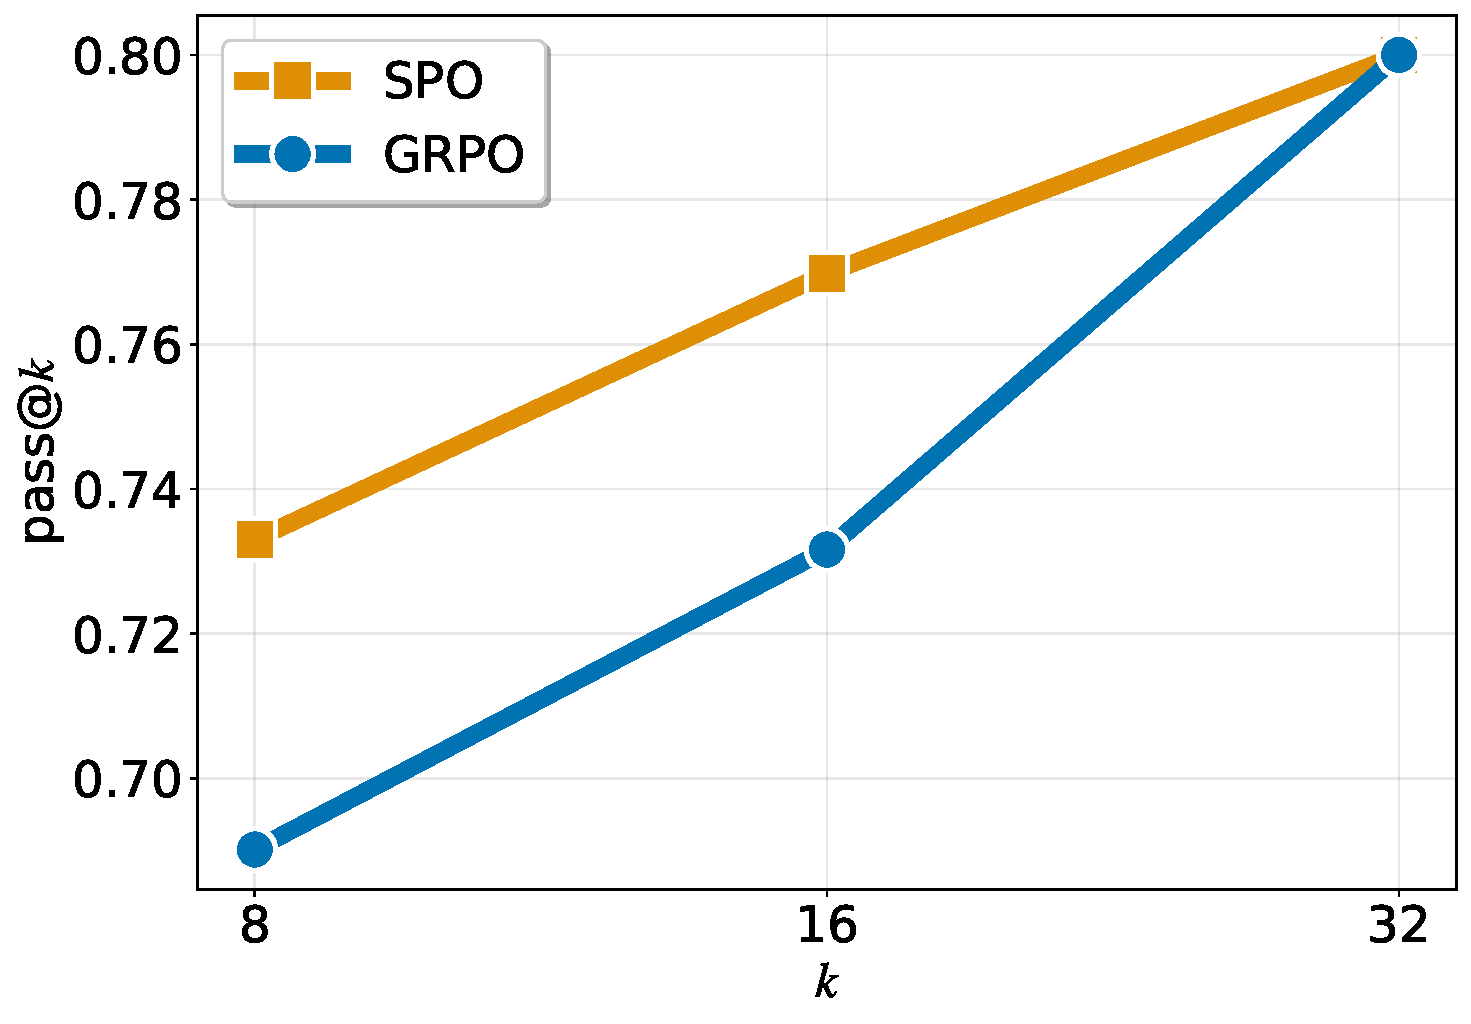
\includegraphics[width=\linewidth]{figures/GRPO_vs_SPO_BRUMO25_pass_at_k.pdf}
  \caption{BRUMO 25}
  \label{fig:pass_k_brumo25}
\end{subfigure}
\hfill
\begin{subfigure}{0.32\textwidth}
  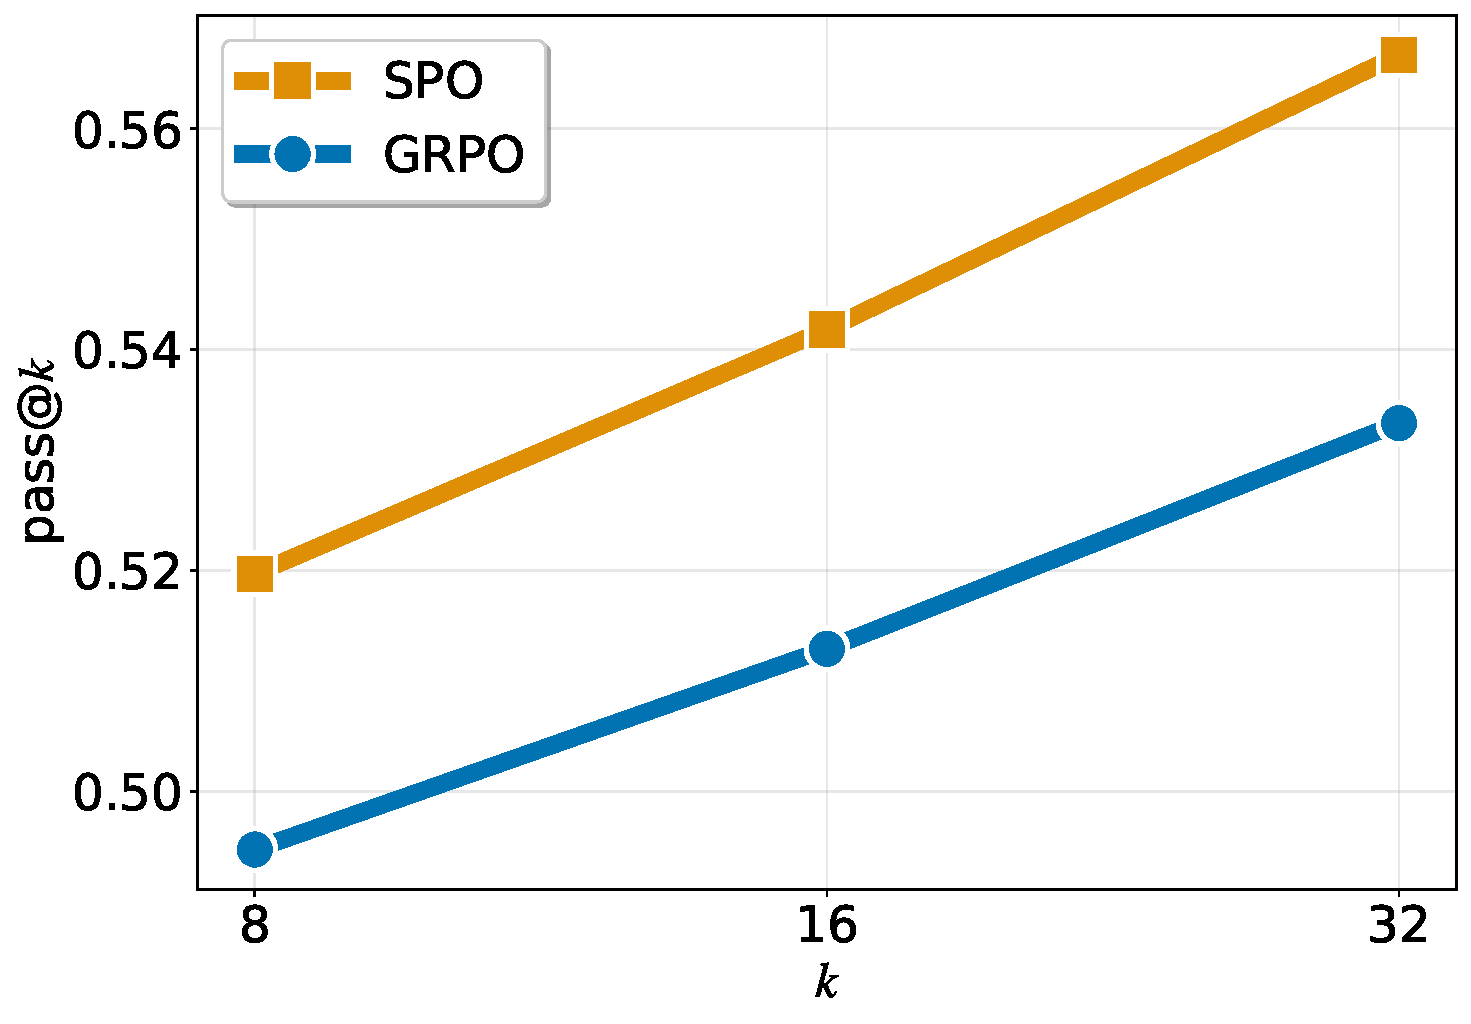
\includegraphics[width=\linewidth]{figures/GRPO_vs_SPO_HMMT25_pass_at_k.pdf}
  \caption{HMMT 25}
  \label{fig:pass_k_hmmt25}
\end{subfigure}
\hfill
\begin{subfigure}{0.32\textwidth}
  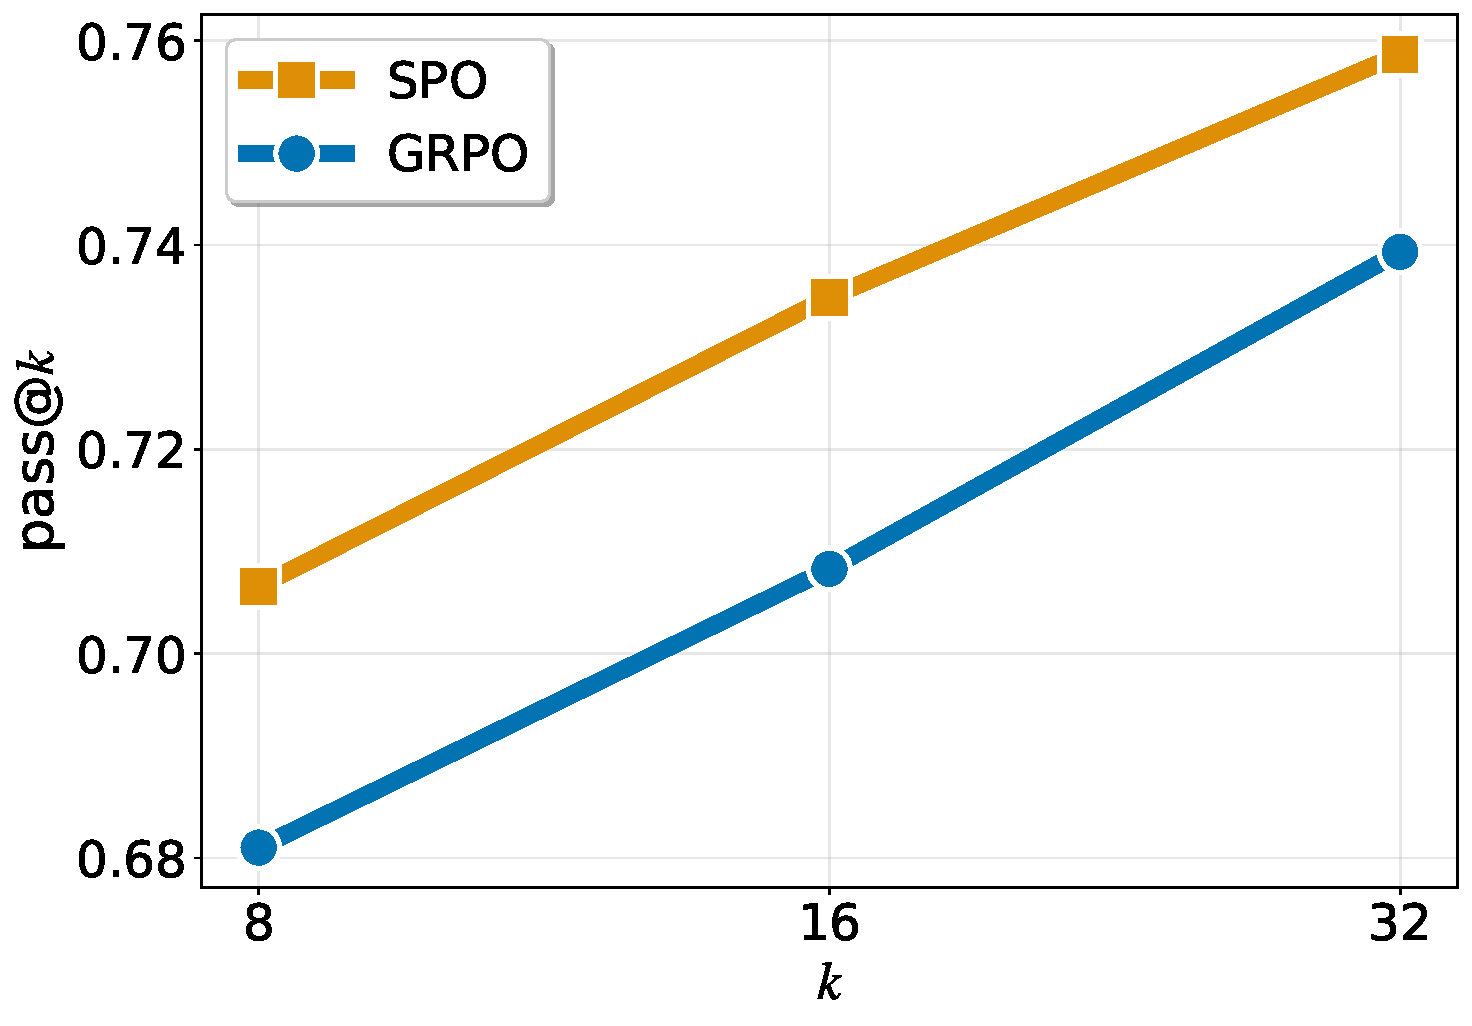
\includegraphics[width=\linewidth]{figures/GRPO_vs_SPO_average_pass_at_k.pdf}
  \caption{Average}
  \label{fig:pass_k_avg}
\end{subfigure}

\end{minipage}%
}
\caption{Pass@$k$ plots comparing GRPO and SPO across five math competition benchmarks.}
\label{fig:pass_k}
\end{figure}

Our experiments demonstrate that SPO outperforms the GRPO baseline on aggregate metrics when training the Qwen-8B model. As shown in Table~\ref{tab:main_results}, SPO achieves superior weighted average scores on both primary metrics. It obtains a maj@32 of $63.8$ compared to GRPO's $60.4$, a significant improvement of $+3.4~\text{percentage points}~(\mathrm{pp})$. This aggregate strength is driven by remarkable consistency, as SPO outperforms GRPO on the maj@32 metric across all five benchmarks. The performance gap is most pronounced on \textbf{BRUMO 25}, where SPO achieves a substantial $+7.3~\mathrm{pp}$ ($64.0$ vs. $56.7$). Further significant gains are seen on \textbf{AIME 25} ($+4.4~\mathrm{pp}$) and \textbf{HMMT 25} ($+3.3~\mathrm{pp}$ points), underscoring the robustness of SPO's improvements. Notably, these benchmarks have minimal data contamination~\citep{matharena}, allowing them to serve as a true test of \emph{generalization}. This demonstrates that our SPO method improves the model's ability to generalize rather than simply overfit to the training data, a risk exemplified by the DAPO dataset's strong correlation with AIME 24.  While GRPO remains competitive on the avg@32 metric in some cases, SPO's consistent and significant advantage in maj@32 suggests it learns more robust and repeatable solutions, a key goal for reliable reasoning models.

These findings are mirrored in the pass@$k$ performance shown in Figure~\ref{fig:pass_k}. The weighted average curve (Figure~\ref{fig:pass_k_avg}) shows a clear and consistent advantage for SPO across all values of $k$, translating to an average improvement of approximately $2.4~\mathrm{pp}$. While the performance on avg@32 is more competitive on a per-benchmark basis, SPO's strong overall performance underscores the stability and effectiveness of its learning signal. We provide additional ablation studies on $A^*$-PO, SPO with no baseline, and SPO with no offline initialization in Appendix~\ref{appendix:ablation}.








\subsection{Analysis of Signal Efficiency and Stability}

\begin{figure}[h!]
    \centering
    \begin{adjustbox}{width=0.8\textwidth, center}
    \begin{minipage}{\textwidth}
    \begin{subfigure}{0.49\textwidth}
        \centering
        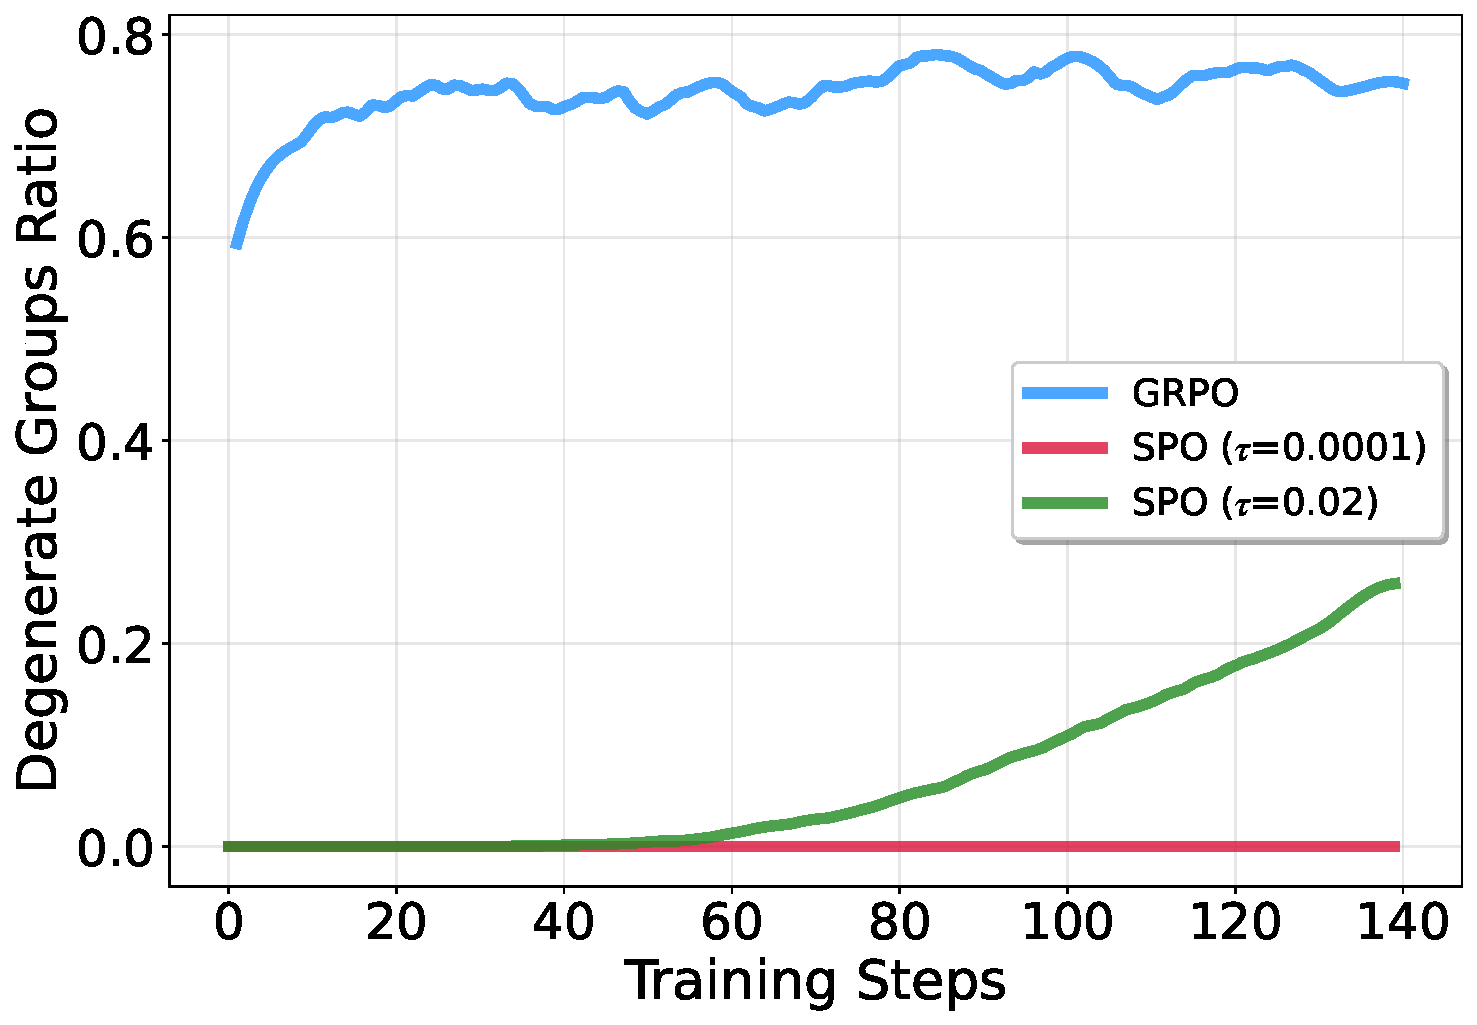
\includegraphics[width=\linewidth]{figures/degenerate_groups_comparison.pdf}
        \caption{Ineffective Gradient Ratios}
        \label{fig:sub_degenerate}
    \end{subfigure}
    \hfill %
    \begin{subfigure}{0.49\textwidth}
        \centering
        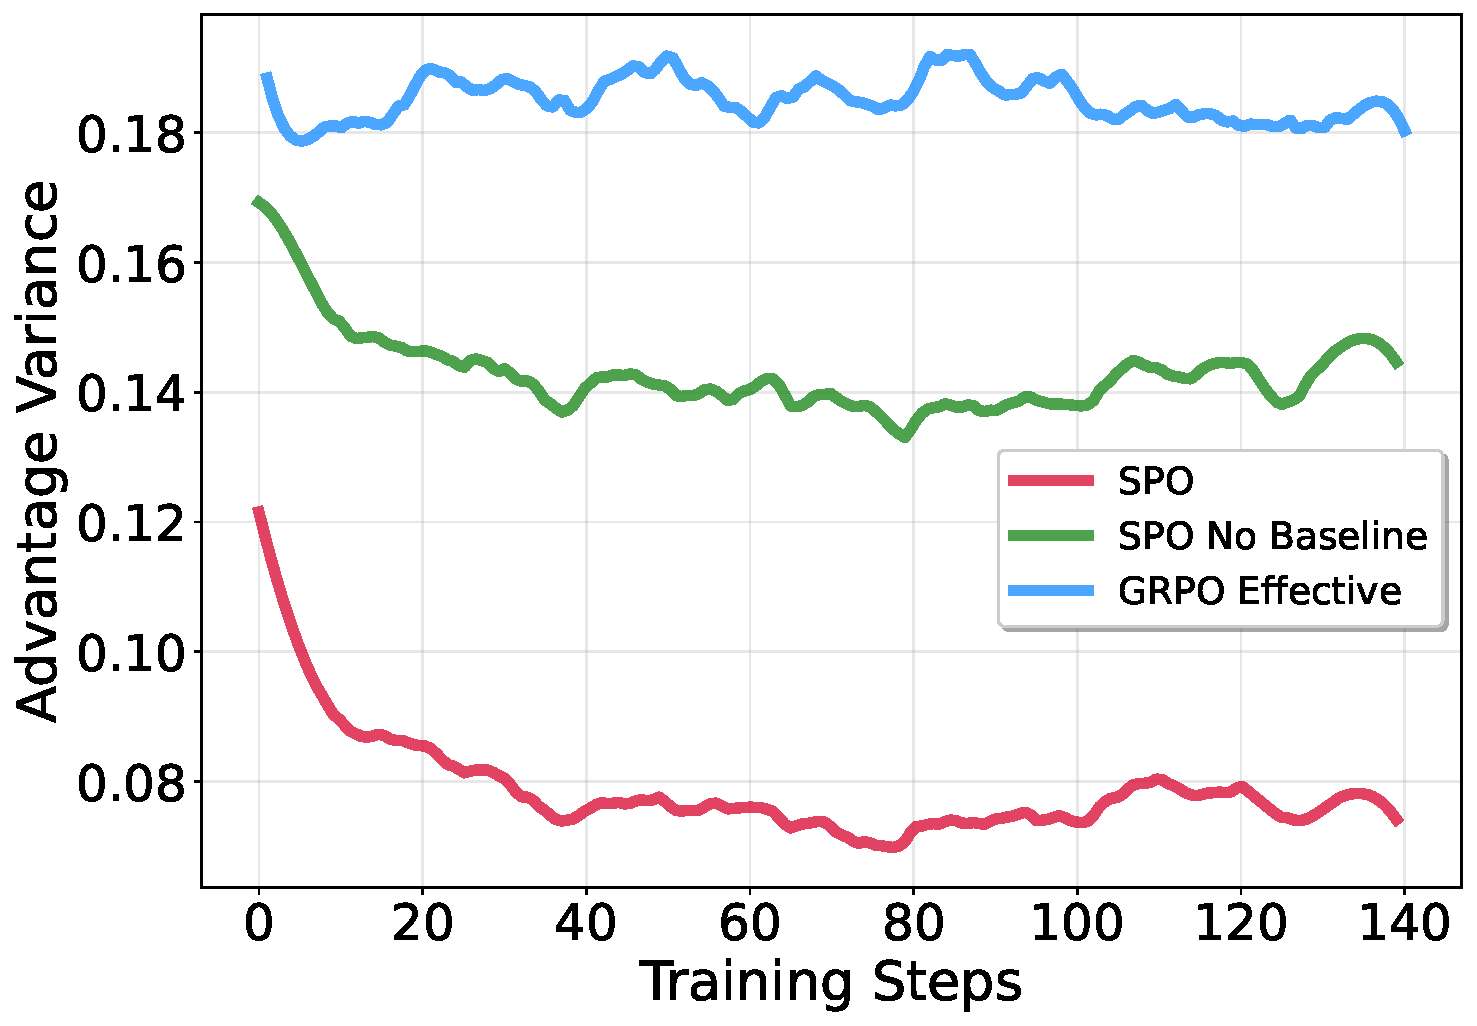
\includegraphics[width=\linewidth]{figures/effective_advantage_variance_comparison.pdf}
        \caption{Advantage Variance Comparison}
        \label{fig:sub_variance}
    \end{subfigure}
    \end{minipage}
    \end{adjustbox}
    \caption{
        Signal Efficiency and Stability Analysis of SPO \emph{vs.} GRPO.
        (a) GRPO suffers from a high ratio of degenerate groups (blue), which yield no learning signal. In contrast, SPO's rate of near-zero advantages (red/green) increases as the model learns, reflecting prediction accuracy rather than wasted computation.
        (b) SPO's baseline (red) provides a stable, low-variance signal, significantly reducing the raw reward variance (green). GRPO's effective advantage (blue), calculated only on non-degenerate samples, is highly volatile and unstable.
    }
    \label{fig:signal_analysis}
\end{figure}

To empirically assess the architectural advantages of SPO, we conduct a two-part analysis of the unnormalized advantage signals produced by SPO and GRPO (Figure~\ref{fig:signal_analysis}). First, we quantify complete signal loss arising from degenerate groups. Second, we measure the variance of the remaining learning signals. Together, these metrics characterize each method’s efficiency and stability.

\textbf{Signal Efficiency and Information Loss.} Figure~\ref{fig:sub_degenerate} reports the fraction of ineffective samples. For GRPO (blue), the share of samples in degenerate groups rises from roughly 60\% to over 80\%, yielding zero advantage and no gradient. For SPO, we instead track the proportion of near-zero advantages under two diagnostic tolerances, $\lvert A \rvert \leq \tau$, with values of $\tau=10^{-4}$ (red) and $\tau=0.02$ (green). Advantages under the tight tolerance $\tau=10^{-4}$ remain rare throughout training (red line), while the $\lvert A \rvert \leq 0.02$ share (green) gradually increases as the value tracker $\hat{v}$ becomes more accurate and residuals shrink on mastered prompts. This trend is expected and desirable: it reflects accurate prediction rather than signal loss. Unlike GRPO’s degenerate groups, these SPO samples are not discarded, they still produce well-defined gradients and contribute to learning. Notably, even under the stricter $\tau=0.02$ tolerance, SPO’s near-zero ratio remains far below GRPO’s degenerate rate, underscoring SPO’s efficient use of compute.

\textbf{Signal Stability and Advantage Variance.} Figure~\ref{fig:sub_variance} compares advantage variance across methods. As a reference, the green line (``SPO No Baseline'') corresponds to raw rewards, i.e., the high-variance signal faced by vanilla policy gradient. SPO’s history-informed baseline (red) delivers a substantial, stable variance reduction of nearly 50\%. For GRPO, computing variance only over non-degenerate samples (``GRPO Effective'', blue) reveals a highly volatile signal with the largest variance among all conditions, exceeding even ``SPO No Baseline''. We conclude that SPO’s baseline is effective, yielding stable, low-variance gradients, whereas GRPO’s on-the-fly baseline is noisy and destabilizing when it produces a signal. The apparent stability of GRPO’s overall variance is driven by the prevalence of zero-variance degenerate samples and thus reflects inefficiency rather than robustness.


\subsection{Agentic Training Demonstrations}
We perform simulations to demonstrate the practical implications of SPO's group-free design in agentic training scenarios, where interaction times can be highly variable. Group-based methods like GRPO suffer from a critical scalability bottleneck due to their inherent synchronization barrier, a problem that is particularly acute in agentic tasks involving multi-turn tool use or long-horizon reasoning.

Figure~\ref{fig:agentic_bottleneck} illustrates this fundamental issue. In an idealized low-variance setting (Figure~\ref{fig:low-variance}), where all agentic trajectories complete in similar times, the group-based approach is efficient. However, in a more realistic high-variance setting (Figure~\ref{fig:high-variance}) characterized by long-tail latencies, a single slow-running trajectory (a ``straggler'') can stall the entire group. In our simulation, while most samples finish in under $133$ seconds, the group must wait $508$ seconds for its slowest member. This bottleneck effect forces faster samples to remain idle, severely hindering training throughput and wasting computational resources.

\begin{figure}[h!]
    \centering
    \begin{adjustbox}{width=0.8\textwidth, center}
    \begin{minipage}{\textwidth}
    \begin{subfigure}{0.45\textwidth}
        \centering
        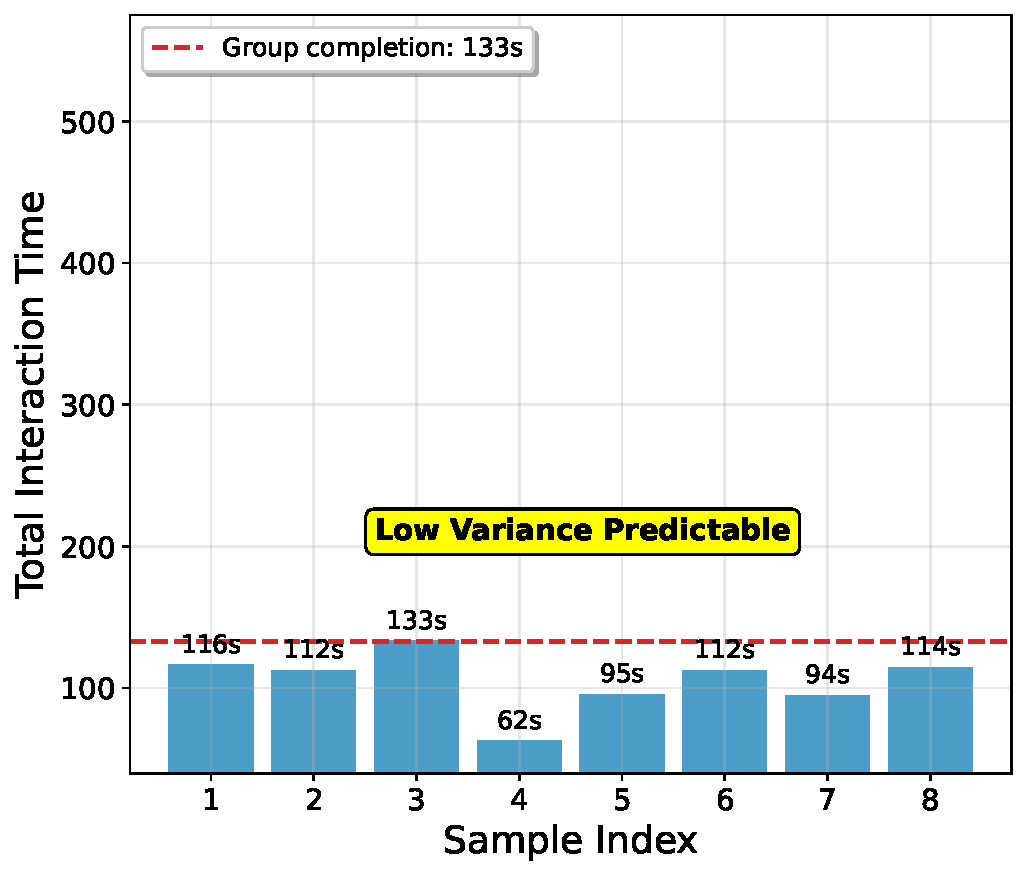
\includegraphics[width=\linewidth]{figures/uniform_distribution.pdf}
        \caption{Low-variance Group}
        \label{fig:low-variance}
    \end{subfigure}
    \hfill %
    \begin{subfigure}{0.45\textwidth}
        \centering
        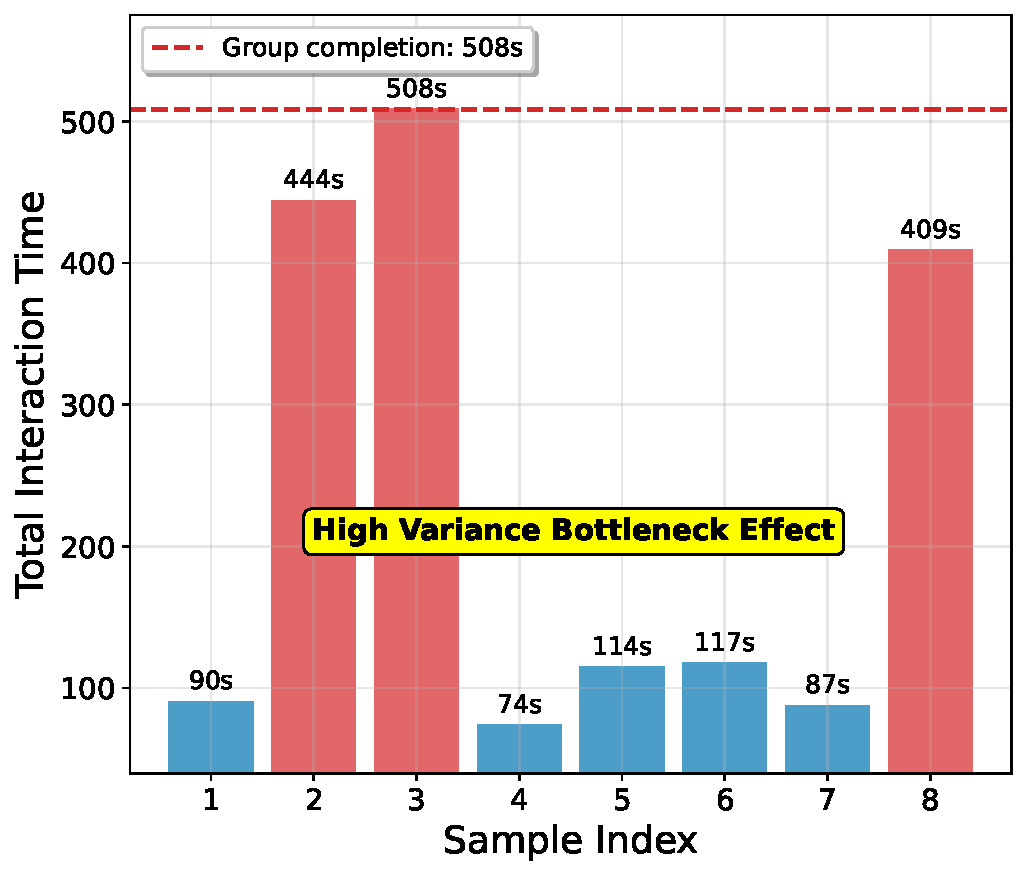
\includegraphics[width=\linewidth]{figures/longtail_distribution.pdf}
        \caption{High-variance Group}
        \label{fig:high-variance}
    \end{subfigure}
    \end{minipage}
    \end{adjustbox}
    \caption{The Bottleneck Effect in Group-Based Sampling. (a) In a low-variance environment, sample completion times are predictable, and the group synchronization cost is minimal. (b) In a realistic high-variance agentic environment, three slow trajectories ($444s$, $508s$, and $409s$) create a severe bottleneck, forcing the entire group to wait and wasting the compute used for the six faster samples.}
    \label{fig:agentic_bottleneck}
\end{figure}

\begin{figure}[h!]
    \centering
    \begin{adjustbox}{width=0.95\textwidth, center}
    \begin{minipage}{\textwidth}
    \begin{subfigure}{0.31\textwidth}
        \centering
        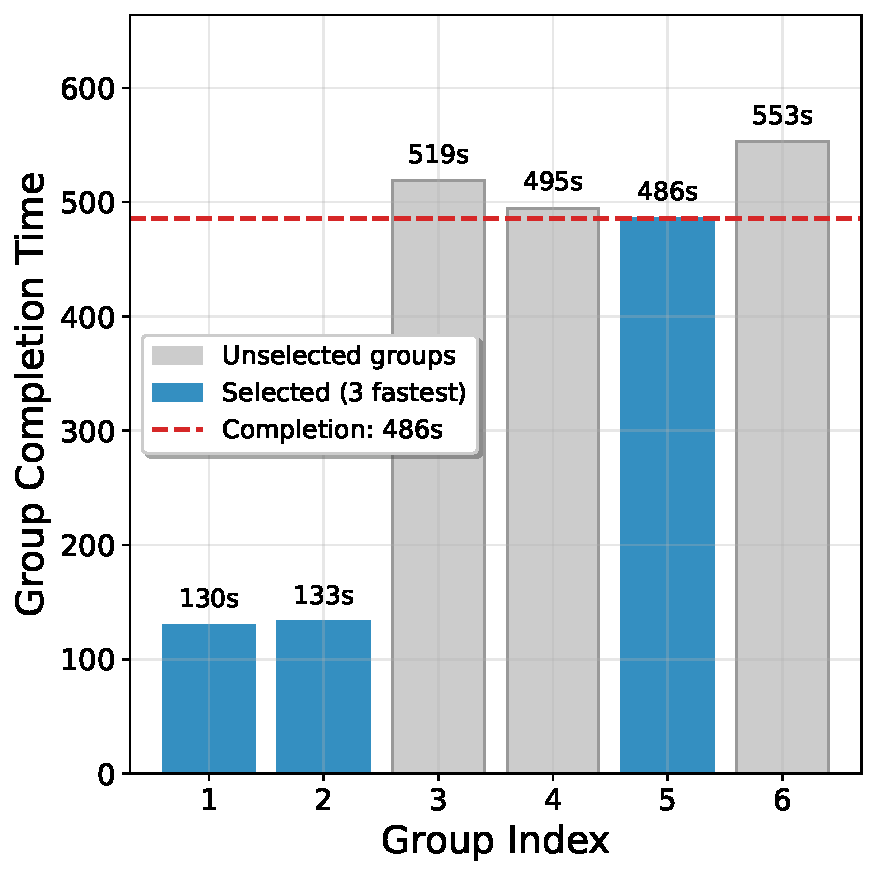
\includegraphics[width=\linewidth]{figures/group_based.pdf}
        \caption{Group-base}
        \label{fig:group_base}
    \end{subfigure}
    \hfill %
    \begin{subfigure}{0.31\textwidth}
        \centering
        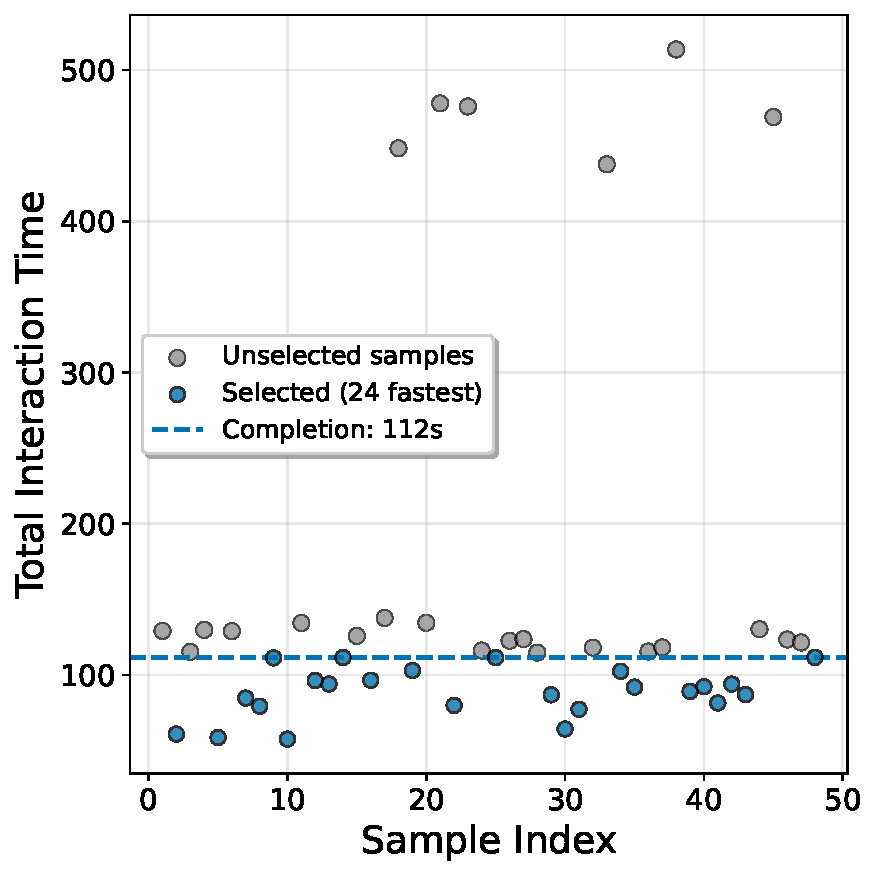
\includegraphics[width=\linewidth]{figures/group_free.pdf}
        \caption{Group-free}
        \label{fig:group_free}
    \end{subfigure}
    \hfill %
    \begin{subfigure}{0.31\textwidth}
        \centering
        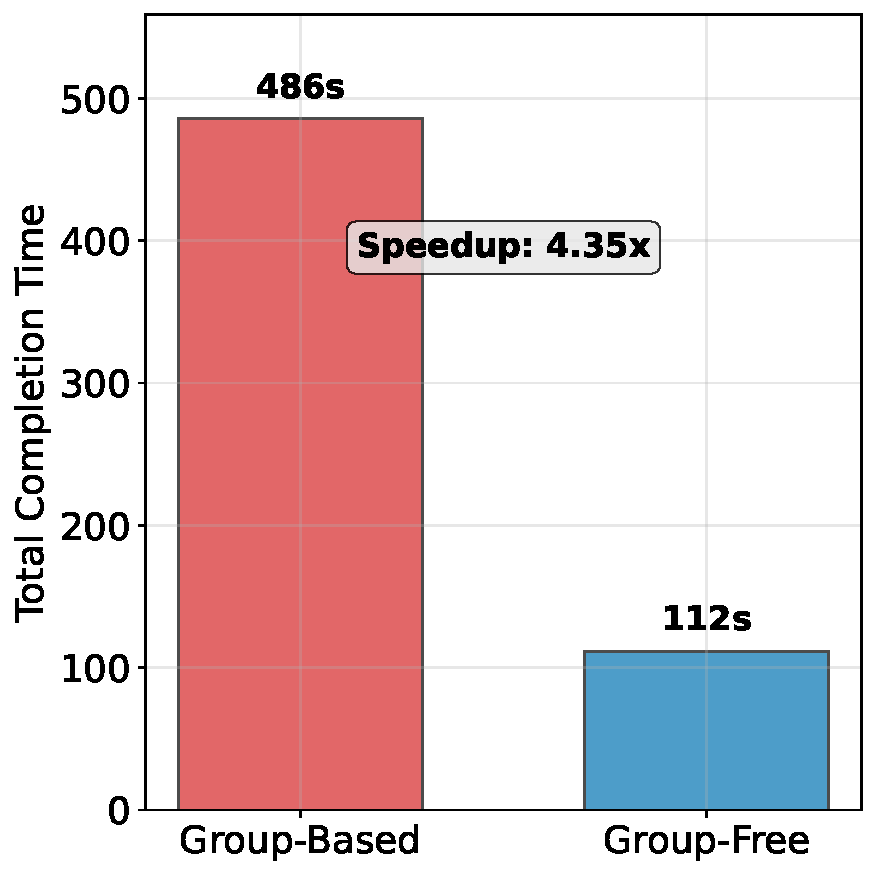
\includegraphics[width=\linewidth]{figures/strategy_comparison.pdf}
        \caption{Strategy Comparison}
        \label{fig:comparison}
    \end{subfigure}
    \end{minipage}
    \end{adjustbox}
    \caption{Throughput Comparison: Group-Based vs. Group-Free. (a) A group-based strategy, even when parallelized, is bottlenecked by its slowest group, taking $486s$ to collect a batch of 3 groups (24 samples). (b) A group-free strategy collects the 24 fastest samples from a larger pool of 48, completing the batch in just $112s$ by avoiding stragglers. (c) The group-free approach achieves a $4.35\times$ speedup, demonstrating its superior efficiency for agentic training.}
    \label{fig:agentic_speedup}
\end{figure}


SPO's group-free architecture directly resolves this inefficiency. Figure~\ref{fig:agentic_speedup} compares the time required to assemble a training batch of 24 samples using both strategies. The group-based approach (left), even when optimized by running 6 groups in parallel and selecting the 3 fastest, is still constrained by the slowest trajectory within those selected groups, taking $486s$ to complete. In contrast, the group-free approach (middle) leverages asynchrony by starting 48 independent samples and simply collecting the first 24 to finish. In our simulated scenario, this process takes only $112s$, as it naturally filters out the slow outliers. As shown on the right, this architectural difference results in a significant $\mathbf{4.35\times}$ speedup in this realistic agentic simulation. Simulations show that SPO's architecture can lead to significant throughput gains, making it a more scalable and robust foundation for training on complex, long-horizon agentic tasks.






















